\section{Algorithms}\label{sec:algorithms}
This chapter describes how scalafmt formats Scala code.
We will see that scalafmt's design is inspired by ClangFormat and dartfmt.
However, we believe our design makes a valuable contribution in that it leverages functional programming principles to maximise code reuse and extensibility.

\subsection{Design}
Figure~\ref{fig:architecture} shows a broad architectural overview of scalafmt.
\begin{figure}
  \centering
  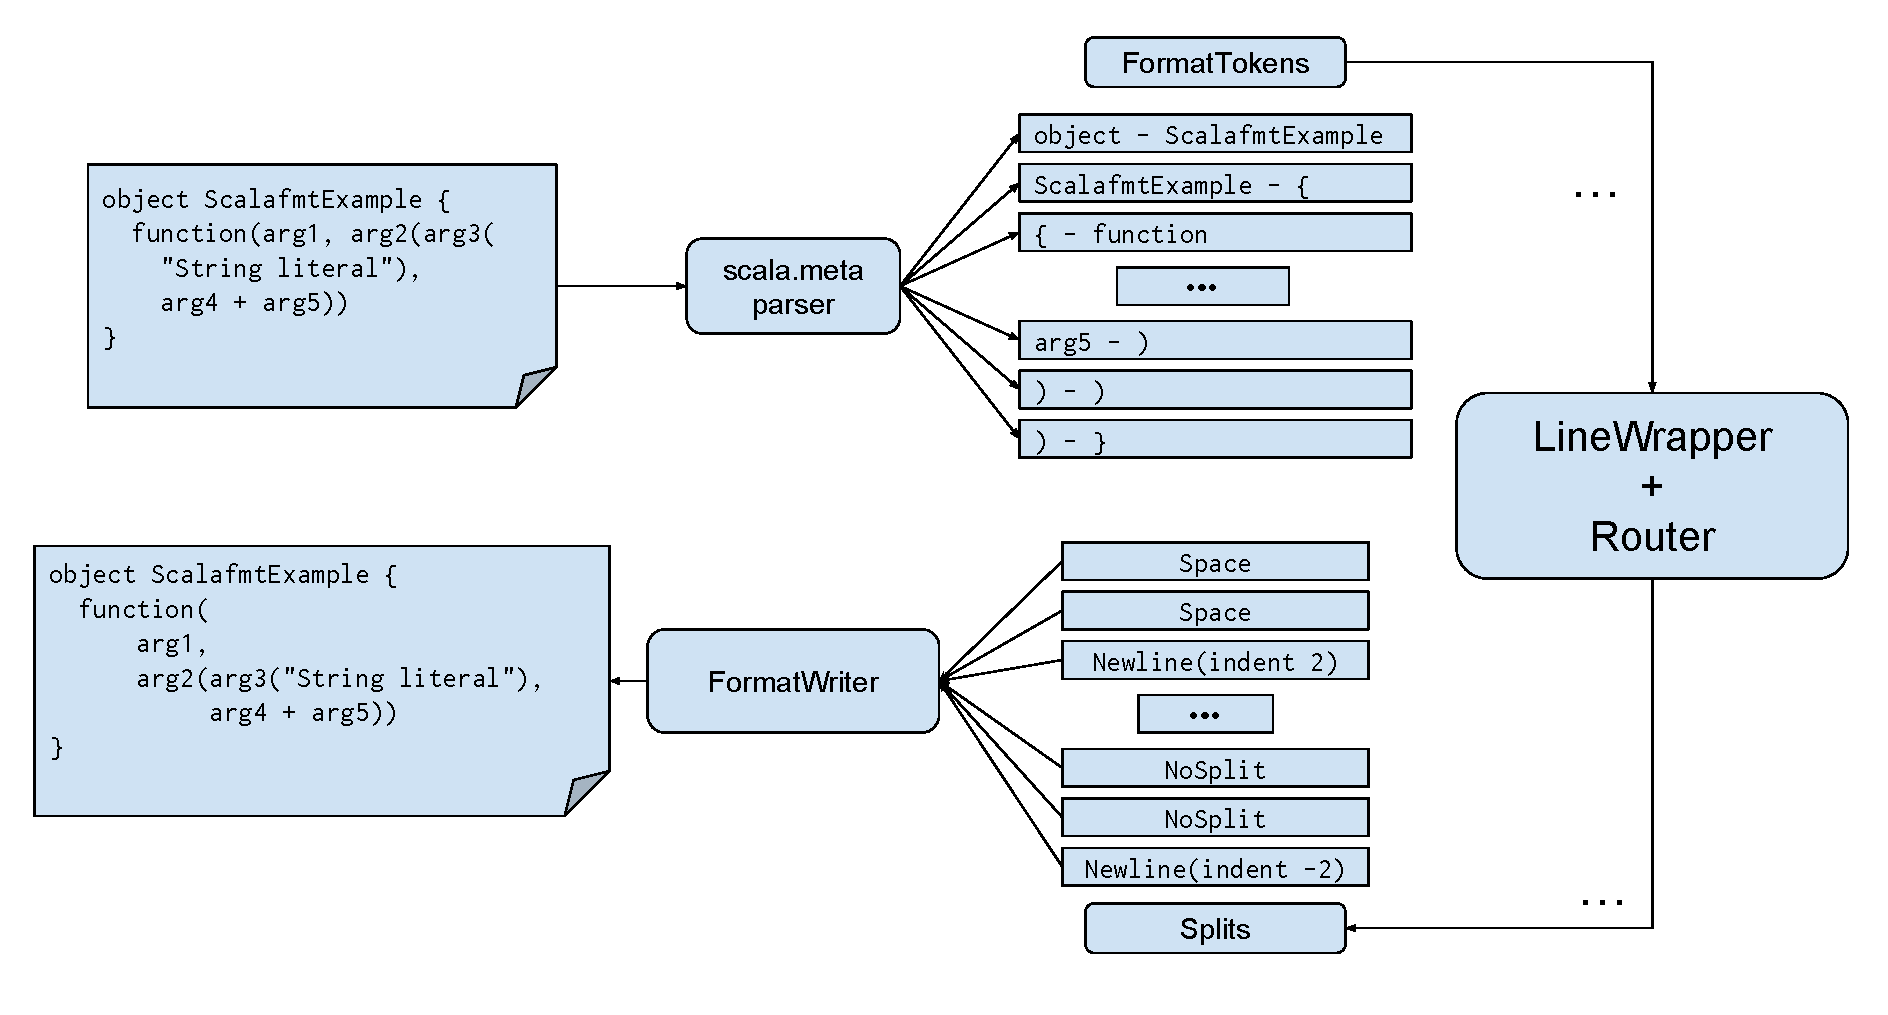
\includegraphics[width=\textwidth]{img/architechture.pdf}
  \caption{Scalafmt architecture}
  \label{fig:architecture}
\end{figure}
First, scalafmt parses a source file using scala.meta.
Next, we feed a sequence of \emph{FormatToken} data types into a \emph{LineWrapper}.
The LineWrapper uses a \emph{Router} to construct a weighted directed graph and run a best-first search to find an optimal formatting layout for the whole file.
Finally, the LineWrapper feeds a sequence of \emph{Split} data types into the \emph{FormatWriter}, which constructs a new reformatted source file.
The following sections explain these data types and abstractions in detail.

\subsection{Data structures}
Scalafmt leverages a few carefully designed data structure to allow an implementation that emphasizes correctness and maintainability.

\subsubsection{FormatToken}
A \emph{FormatToken} is a pair of two non-whitespace tokens.
Listing~\ref{lst:format_token} shows the definition of the FormatToken data type.
\lstinputlisting[label={lst:format_token}, caption=FormatToken definition]{code/format_token.scala}
As shown in the architecture overview in figure~\ref{fig:architecture}, each token except the beginning and end of file tokens appear twice in the sequence of FormatTokens: once as the \texttt{left} member and once as the \texttt{right} member.
In a nutshell, the job of the LineWrapper is to convert each FormatToken into a \emph{Split}

\subsubsection{Decision}\label{sec:decision}
A Decision is a pair of a FormatToken and a sequence of Splits.
Listing~\ref{lst:decision} shows the Definition of decision.
\lstinputlisting[label={lst:decision}, caption=Decision definition]{code/decision.scala}
The \emph{splits} member represents the possible splits that we can take at \emph{formatToken}.

\subsubsection{Policy}\label{sec:policy}
A \emph{Policy} is an enforced formatting layout over a region.
Listing~\ref{lst:policy} shows the definition of Policy.
\begin{minipage}{\linewidth}
  \lstinputlisting[label={lst:policy}, caption=Policy definition]{code/policy.scala}
\end{minipage}
A Policy is a partial function that should be applied to future Decisions up until the \emph{expire} token.
Policies easily compose using the Scala standard library \texttt{orElse} and \texttt{andThen} methods on PartialFunction\footnote{
  Careful eyes will observe that Policy is in fact a monoid with the empty partial function as identity and function composition as associative operator.}.
This enables a high-level way to express arbitrary formatting layouts over a region of code.

\subsubsection{Indent}\label{sec:indent}
An \emph{Indent} describes indentation over a region of code.
\lstinputlisting[label={lst:indent}, caption=Indent definition]{code/indent.scala}
Listing~\ref{lst:indent} shows the definition of Indent along with the algebraic data type \emph{Length}.
Length can either be \texttt{Num(n)} where $n$ represents an explicit number of spaces to indent by or \texttt{StateColumn} which is a placeholder the number of spaces required to vertically align by the current column.
Indent is type parameterized by Length so that, at some point, we can replace StateColumn placeholders with Nums to obtain a concrete number.
For example, given a scala.meta tree \texttt{expr}, the definition \texttt{Indent(Num(2), expr.tokens.last, inclusive=true)}
increases the indentation level by 2 spaces up to and including the last token of \texttt{expr}.
The \texttt{inclusive} member is set to false when the indentation should expire before the expire token, for example in a block wrapped by curly braces, since the closing curly brace should not be indented by 2 spaces.
The StateColumn placeholder is required to allow memoization of Splits, which is critical for performance reason as explained in section~\ref{sec:router} on the \emph{Router}.

\subsubsection{Split}
A \emph{Split} represents a (possibly empty) whitespace character to be inserted between two non-whitespace tokens.
Listing~\ref{lst:split} shows the rather intricate definition of the Split data type\footnote{
  For clarity reasons, a few less important members have been removed from the actual Split definition.}.
\begin{minipage}{\linewidth}
  \lstinputlisting[label={lst:split}, caption=Split definition]{code/split.scala}
\end{minipage}
The Split data type went through several generations of design before reaching its current structure.
Each member serves an important role.
The most important member of the Split type is the \emph{modification}.
A modification must be one of \texttt{NoSplit}, \texttt{Space} and \texttt{Newline}.
The \emph{cost} member represents the penalty for choosing this split.
The \emph{optimalToken} member enables an optimization explained in section~\ref{sec:optimal}.
The \emph{indents} member contains the indentation layers that this splits adds.
The \emph{line} member allows a powerful debugging technique explained in section~\ref{sec:line}.
The \emph{policy} and \emph{indents} members are explained in sections~\ref{sec:policy} and~\ref{sec:indent}, respectively.

\subsection{LineWrapper}
The LineWrapper is responsible for turning FormatTokens into Splits.
To accomplish this, the LineWrapper employs a \emph{Router} and abest-first search.

\subsubsection{Router}\label{sec:router}
The Router's role is to produce a Decision given a FormatToken.

There can be a lot of 
How do we go about implementing a Router?

By producing Decisions, the Router constructs a weighted directed graph that represents all possible formatting layouts for an input source code.
Figure~\ref{fig:router} shows a simplified graph for the input \texttt{val x = y + z}.
\begin{figure}
  \centering
  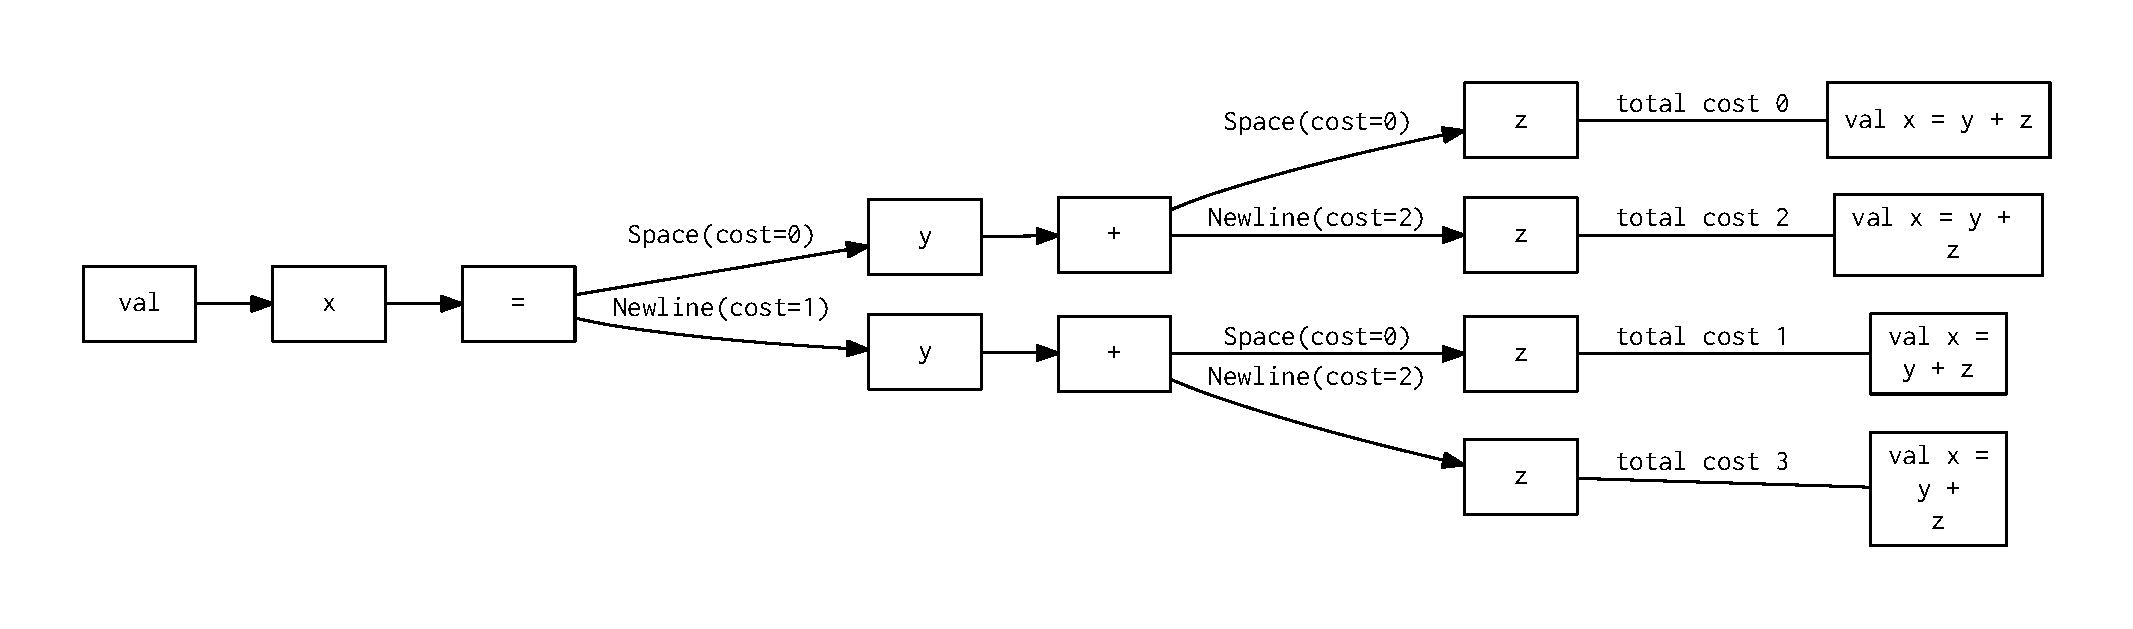
\includegraphics[width=\textwidth]{target/router.pdf}
  \caption{Weighted directed graph}
  \label{fig:router}
\end{figure}
Figure is simplified for clarity reason.
For example, the actual scalafmt implementation adds policies and indentations after the assignment operator.
In a nutshell, a router is a function from FormatToken to Decision.



\subsubsection{BestFirstSearch}
Observe that graph in listing~\ref{fig:router} grows exponentially at every FormatToken where we have more than one Split options.
If we implement the best first search \naive{}ly
This must be handled intelligently by the best-first search.

\subsection{Optimizations}
\subsubsection{OptimalToken}\label{sec:optimal}
\subsubsection{dequeueOnNewStatements}
\subsubsection{recurseOnBlocks}
\subsubsection{escapeInPathologicalCases}
\subsubsection{escapeInPathologicalCases}
\subsubsection{pruneSlowStates}
\subsubsection{FormatWriter}
\begin{itemize}
  \item vertical alignment
  \item comment formatting
  \item stripMargin alignment
\end{itemize}
